%-----------------------------------------------------------------------
%
%   UFRJ  - Universidade Federal do Rio de Janeiro
%   COPPE - Coordena��o dos Programas de P�s-gradua��o em Engenharia
%   PEE   - Programa de Engenharia El�trica
%
%
%   Projeto ROSA - Rob� para opera��o de stoplogs alagados
%
%   Minutas de reuni�es
%
%                                                        20/mar/14, Rio
%                                                        Ramon R. Costa
%----------------------------------------------------------------------
\documentclass[12pt,a4paper]{article}
\usepackage{amsmath,amssymb}  %pacotes do AMS
\usepackage[utf8]{inputenc} %pacote para entender palavras acentuadas
\usepackage{latexsym}         %pacote para incluir simbolos (ex.\Box)
\usepackage{fancybox,fancyhdr}%pacote com frescuras
\usepackage{graphicx}         %pacote para incluir figuras tipo eps
\usepackage{xcolor}
\usepackage{xspace}
\usepackage{pst-all,pst-poly}  %PSTricks
\usepackage{psfrag}
\usepackage{calc}
\usepackage{multicol}
\usepackage[english]{babel} 
\usepackage[a4paper]{hyperref}

 
%----------------------------------------------------------------------
%
%   Macros utilizados no LATEX.
%                                                       Ramon R. Costa
%                                                       23/jun/94, Rio
%----------------------------------------------------------------------
\newcount\m
\newcount\n

\def\twodigits#1{\ifnum #1<10 0\fi \number#1}

\def\hours{\n=\time \divide\n 60
    \m=-\n \multiply\m 60 \advance\m \time
    \twodigits\n:\twodigits\m}

\def\hora{\hours}

\def\data{Rio de Janeiro,\  \number\day\  de \ifcase\month\or
    janeiro\or
    fevereiro\or
    mar\c{c}o\or
    abril\or
    maio\or
    junho\or
    julho\or
    agosto\or
    setembro\or
    outubro\or
    novembro\or
    dezembro\or\fi\  de \number\year}

%----------------------------------------------------------------------

\newcommand{\bl}{\begin{itemize}}           %item point
\newcommand{\el}{\end{itemize}}

\newcommand{\blista}{
    \vspace{-1.5ex}
    \begin{itemize}
    \renewcommand{\labelitemi}{$\Box$}
    \setlength {\itemsep}{-0.8mm}
    \setlength {\parsep} {0mm}
    }

\newcommand{\elista}{
    \end{itemize}
    \vspace{-1ex}
    }

\newcommand{\bd}{\begin{description}}       %item simples
\newcommand{\ed}{\end{description}}

\newcommand{\bn}{\begin{enumerate}}     %item numero
\newcommand{\en}{\end{enumerate}}

\newcommand{\figps}[4]{
    \begin{figure}[htb]
    \centerline{
    \psfig{figure = #4, height = #1cm}
    }
    \caption{#2}
    \label{#3}
    \end{figure}
    }

\newcommand{\mfig}[5]{
    \begin{figure}[htb]
    \centerline{
    \psfig{figure=#5, height=#1cm, width=#2cm}
    }
    \caption{#3}
    \label{#4}
    \end{figure}
    }

\newcommand{\bvect}{\left(\begin{array}{c} }

\newcommand{\evect}{\end{array}\right)}

\newcommand{\mat}[1]{
    \left[
    \begin{array}   % \mat{{cclr} 1&2&3&4 \\ 1&1&1&1}
        #1
    \end{array}
    \right]
}

\newcommand{\matriz}[1]{    %Latex 2e + amstex
    \begin{bmatrix}
        #1
    \end{bmatrix}
}

\newcommand{\equ}[2]{                      % \equ{equation}{label}
  \begin{equation}\label{#2}
  #1
  \end{equation}
}

\newcommand{\dequ}[3]{
    \addtolength{\arraycolsep}{-1mm}
    \renewcommand{\arraystretch}{1.4}
    \begin{equation}
        \begin{array}{rcl}
            #1 \nonumber \\
            #2 \nonumber
        \end{array}
        \label{#3}
    \end{equation}
    \renewcommand{\arraystretch}{1}
    \addtolength{\arraycolsep}{1mm}
}

\newcommand{\tequ}[4]{
    \addtolength{\arraycolsep}{-1mm}
    \renewcommand{\arraystretch}{1.4}
    \begin{equation}
        \begin{array}{rcl}
            #1 \nonumber \\
            #2 \nonumber \\
            #3 \nonumber
        \end{array}
        \label{#4}
    \end{equation}
    \renewcommand{\arraystretch}{1}
    \addtolength{\arraycolsep}{1mm}
}

\newcommand{\cequ}[4]{
    %\addtolength{\arraycolsep}{-1mm}
    \renewcommand{\arraystretch}{1.4}
    \begin{equation}
        #1 = \left\{
        \begin{array}{lcl}
            #2  \\
            #3
        \end{array}
        \right.
        \label{#4}
    \end{equation}
    \renewcommand{\arraystretch}{1}
    %\addtolength{\arraycolsep}{1mm}
}

\newcommand{\eqn}[1]{                      % \equ{equation}{nolabel}
        \begin{equation}
        #1
        \end{equation}
}

\newcommand{\espacoduplo}{\setlength{\baselineskip}{1.5\baselineskip}}
\newcommand{\espacosimples}{\setlength{\baselineskip}{.7\baselineskip}}

\newcommand{\mref}[1]{(\ref{#1})}

%----------------------------------------------------------------------
%
% Agregado por Fernando.
%

\newcommand{\cents}{\hbox{\rm\rlap/c}}
\newcommand{\abs}[1] {\left|#1\right|}
\newcommand{\norm}[1] {\left|\!\left|#1\right|\!\right|}
\newcommand{\vvert}{\Vert}       %always translated to \left| or \right|

%\newcount\notenumber
%\newcommand {\clearnotenumber}{\notenumber=0}
% \newcommand {\note}{\global\advance\notenumber by 1
% \footnote{$^{\the\notenumber}$}}
%\clearnotenumber
%\indice{variavel}{indice}

\newcommand{\indice}[2]{
    #1_{\scriptscriptstyle #2}
}

\newcommand{\espfig}[3]{
        \begin{figure}[htb]
        \vspace{#1cm}
        \caption{{#2}}
        \label{#3}
        \end{figure}
}

\newcommand{\mkfig}[5]{
    \begin{figure}[htb]
        \centerline{
            \psfig{figure=#1.ps,height=#2cm,width=#3cm}
        }
        \caption{{#4}}
        \label{#5}
    \end{figure}
}

%derivee partielle (attention se mettre en mode math)
\newcommand{\dpar}[2]{
    {\frac {\partial #1}{\partial #2}}
}

%derivee partielle (attention se mettre en mode math)
\newcommand{\dnpar}[3]{
    {\frac {\partial ^{#3}#1}{\partial #2^{#3}}}
}

%derivee normale (etre en mode math)
\newcommand{\deriv}[2]{
    {\frac {d #1}{d #2}}
}

\newcommand{\derivn}[2]{
    {\frac {d^{#2}#1}{dt^{#2}}}
}

%----------------------------------------------------------------------
%
% Agregado por Ramon.
%

\newcommand{\CAO}{\c{C}\~{A}O}
\newcommand{\cao}{\c{c}\~{a}o}

\newcommand{\COES}{\c{C}\~{O}ES}
\newcommand{\coes}{\c{c}\~{o}es}

\newcommand{\pee}{Programa de Engenharia El\a'etrica}
\newcommand{\PEE}{PROGRAMA DE ENGENHARIA EL\a'ETRICA}

\newcommand{\coppe}{Coordena\cao\ dos Programas de P\a'os--Gradua\cao\ em Engenharia}
\newcommand{\COPPE}{COORDENA\CAO\ DOS PROGRAMAS DE P\a'OS--GRADUA\CAO\ EM ENGENHARIA}

\newcommand{\ct}{Centro de Tecnologia}
\newcommand{\CT}{CENTRO DE TECNOLOGIA}

\newcommand{\ufrj}{Universidade Federal do Rio de Janeiro}
\newcommand{\UFRJ}{UNIVERSIDADE FEDERAL DO RIO DE JANEIRO}

\newcommand{\rrc}{Ramon Romankevicius Costa}
\newcommand{\RRC}{RAMON ROMANKEVICIUS COSTA}

\newcommand{\ceq}{Comiss\~ao de Exame de Qualifica\cao}
\newcommand{\CEQ}{COMISS\~AO DE EXAME DE QUALIFICA\CAO}

\newcommand{\gscar}{Gru\-po de Si\-mu\-la\-\cao\ e Con\-tro\-le em
            Auto\-ma\-\cao\ e Ro\-b\a'o\-ti\-ca}
\newcommand{\GSCAR}{GRUPO DE SIMULA\CAO\ E CONTROLE EM AUTOMA\CAO\ e ROB\a'OTICA}

\newcommand{\rov}{Ro\-b\^o Sub\-ma\-ri\-no de Ope\-ra\-\cao\ Re\-mo\-ta}
\newcommand{\ROV}{ROB\^O SUBMARINO DE OPERA\CAO\ REMOTA}

\newcommand{\ramon}{
  \vspace{1.5cm}
  \hfill
  \parbox{8cm}{
    \centering
    \rule[0mm]{6cm}{0.1mm} \\[3mm]
    Ramon Romankevicius Costa \\
  }
}

\newcommand{\chefe}{
    \vspace{1.5cm}
    \hspace{7cm}
    \parbox{7cm}{
    \begin{center}
        \rule[0mm]{6cm}{0.1mm} \\
        \vspace{3mm}
        \rrc\\
        \vspace{3mm}
        Chefe da \a'Area de Controle \\
        \pee
    \end{center}}}

\newcommand{\vice}{
    \vspace{1.5cm}
    \hspace{7cm}
    \parbox{7cm}{
    \begin{center}
        \rule[0mm]{6cm}{0.1mm} \\
        \vspace{3mm}
        \rrc\\
        \vspace{3mm}
        Vice--Coordenador \\
        \pee
    \end{center}}}

\newcommand{\coordenador}{
    \vspace{1.5cm}
    \hspace{7cm}
    \parbox{7cm}{
    \begin{center}
        \rule[0mm]{6cm}{0.1mm} \\
        \vspace{3mm}
        \rrc\\
        \vspace{3mm}
        Coordenador \\
        \pee
    \end{center}}}

\newcommand{\orientador}{
    \vspace{1.5cm}
    \hspace{7cm}
    \parbox{7cm}{
    \begin{center}
        \rule[0mm]{6cm}{0.1mm} \\
        \vspace{3mm}
        \rrc\\
        \vspace{3mm}
        Orientador
    \end{center}}}

\newcommand{\liu}{
    \vspace{1.5cm}
    \hfill
    \parbox{8cm}{
    \begin{center}
        \rule[0mm]{6cm}{0.1mm} \\
        \vspace{3mm}
        Liu Hsu \\
%        \vspace{3mm}
%        Chefe do Laborat\'orio de Controle \\
%        \pee
    \end{center}}}

\newcommand{\xEndereco}{
    \vfill
    \begin{small}
    \begin{tabbing}
    Endere\c{c}o :\ \ \= \rrc \\
        \> COPPE/UFRJ --- \pee \\
        \> Caixa Postal 68504 --- CEP 21945--970 --- Rio de Janeiro --- RJ \\
        \> e-mail: {\tt ramon@coep.ufrj.br} \qquad       Fax: 290-6626
    \end{tabbing}
    \end{small}}

\newcommand{\meuendereco}{
    \vfill
    \noindent\rule[0mm]{\textwidth}{0.1mm}
    {\scriptsize \sf
    \begin{minipage}{1.5cm}
        Endere�o :
    \end{minipage}
    \begin{minipage}[t]{8.5cm}
        \rrc\\
        COPPE/UFRJ --- \pee\\
        Caixa Postal 68504 --- CEP 21945--970 --- Rio de Janeiro --- RJ
    \end{minipage}
    \hfill
    \begin{minipage}[t]{4cm}
        \begin{tabbing}
        e-mail\ \= : {\tt ramon@coep.ufrj.br}\\
        Fone    \> : 260-5010 r.267\\
        Fax     \> : 290-6626
        \end{tabbing}
    \end{minipage}
    }}

\newcommand{\laranjeiras}{
    \vfill
    \noindent\rule[0mm]{\textwidth}{0.1mm}
    {\scriptsize \sf
    \begin{minipage}{1.5cm}
        Endere�o :
    \end{minipage}
    \begin{minipage}[t]{8.5cm}
        \rrc\\
        Rua das Laranjeiras, 192/201 \\
        Laranjeiras, CEP 22240--001 --- Rio de Janeiro --- RJ
    \end{minipage}
    \hfill
    \begin{minipage}[t]{4cm}
        \begin{tabbing}
        e-mail\ \= : {\tt ramon@coep.ufrj.br}\\
        Fone    \> : 2265-5520
        Cel.    \> : 9355-8056
        \end{tabbing}
    \end{minipage}
    }}

\newcommand{\Liuendereco}{
    \vfill
    \noindent\rule[0mm]{16.5cm}{0.1mm}
    {\scriptsize \sf
    \begin{minipage}{1.5cm}
        Endere\c{c}o :
    \end{minipage}
    \begin{minipage}[t]{8.5cm}
        Liu Hsu\\
        COPPE/UFRJ --- \pee\\
        Caixa Postal 68504 --- CEP 21945--970 --- Rio de Janeiro --- RJ
    \end{minipage}
    \hfill
    \begin{minipage}[t]{4cm}
        \begin{tabbing}
        e-mail\ \= : {\tt liu@coep.ufrj.br}\\
        Fax     \> : 290-6626
        \end{tabbing}
    \end{minipage}
    }}

\newcommand{\address}{
    \vfill
    \noindent\rule[0mm]{16.5cm}{0.1mm}
    {\scriptsize \sf
    \begin{minipage}{2.3cm}
        Mailing address :
    \end{minipage}
    \begin{minipage}[t]{8.5cm}
        \rrc\\
        COPPE/UFRJ --- Department of Electrical Engineering \\
        P.O. Box 68504 --- 21945--970 --- Rio de Janeiro --- BRAZIL
    \end{minipage}
    \hfill
    \begin{minipage}[t]{4cm}
        \begin{tabbing}
        e-mail\ \= : {\tt ramon@coep.ufrj.br}\\
        Fax     \> : 055 21 290-6626
        \end{tabbing}
    \end{minipage}
    }}

\newcommand{\liuaddress}{
    \vfill
    \noindent\rule[0mm]{16.5cm}{0.1mm}
    {\scriptsize \sf
    \begin{minipage}{2.3cm}
        Mailing address :
    \end{minipage}
    \begin{minipage}[t]{8.5cm}
        Liu Hsu \\
        COPPE/UFRJ --- Department of Electrical Engineering \\
        P.O. Box 68504 --- 21945--970 --- Rio de Janeiro --- BRAZIL
    \end{minipage}
    \hfill
    \begin{minipage}[t]{4cm}
        \begin{tabbing}
        e-mail\ \= : {\tt liu@coep.ufrj.br}\\
        Fax     \> : 290-6626
        \end{tabbing}
    \end{minipage}
    }}

\newcommand{\remetente}{
    \vspace{3cm}
    \parbox{15cm}{
        \rrc \\
        COPPE/UFRJ --- \pee \\
        Caixa Postal 68.504 --- CEP 21.945--970 --- Rio de Janeiro --- RJ
    }
}

\newcommand{\deliver}{
    \vspace{3cm}
    \parbox{15cm}{
        \rrc \\
        COPPE/UFRJ --- Department of Electrical Engineering \\
        P. O. Box 68504 --- 21945--970 --- Rio de Janeiro --- BRAZIL
    }
}

\newcommand{\astrom}{{\AA }str\"{o}m}
\newcommand{\AeW}{\astrom\ \& Wittenmark}
\newcommand{\AeH}{\astrom\ \& H\"agglund}

\newcommand{\fim}{
    \medskip
    \begin{center}
    \rule[1mm]{30mm}{0.14mm}$\diamond$\rule[1mm]{30mm}{0.14mm}
    \end{center}}

\newcommand{\DO}[1]{
    \noindent
    \makebox[8mm][l]{\bf Do }: \parbox[t]{15cm}{#1}

    \smallskip}

\newcommand{\AO}[1]{
    \noindent
    \makebox[8mm][l]{\bf Ao }: \parbox[t]{15cm}{#1}

    }

\newcommand{\AOS}[1]{
    \noindent
    \makebox[8mm][l]{\bf Aos}: \parbox[t]{15cm}{#1}

    }

\newcommand{\A}[1]{
    \noindent
    \makebox[8mm][l]{\bf \`A }: \parbox[t]{15cm}{#1}

    }

\newcommand{\ASSUNTO}[1]{
    \vspace{8mm}
    \noindent
    \hfill {\bf Ref.:} {#1}

    \vspace{5mm}
    }

\newcommand{\diretor}{
    \vspace{1.5cm}
    \hspace{7cm}
    \parbox{7cm}{
    \begin{center}
        \rule[0mm]{6cm}{0.1mm} \\
        \vspace{3mm}
        Prof. Luiz Pinguelli Rosa \\
        \vspace{3mm}
        Diretor da COPPE
    \end{center}}}

%----------------------------------------------------------------------

%----------------------------------------------------------------------
%
%
%     A4 paper size & margins
%
%                                                         Ramon R Costa
%                                                         aug/06/00, SB
%----------------------------------------------------------------------

\setlength {\textheight}    {25cm}%
\setlength {\textwidth}     {17.5cm}%
\setlength {\parindent}     {0mm}%
\setlength {\parskip}       {1mm}%
\setlength {\topmargin}     {-14mm}%
\setlength {\oddsidemargin} {-6mm}%
\setlength {\evensidemargin}{-6mm}%
\setlength {\columnsep}     {6mm}%

%----------------------------------------------------------------------
 
%-----------------------------------------------------------------------
%
%   UFRJ  - Universidade Federal do Rio de Janeiro
%   COPPE - Coordena��o dos Programas de P�s-gradua��o em Engenharia
%   PEE   - Programa de Engenharia El�trica
%
%
%   Projeto ROSA - Rob� para opera��o de stoplogs alagados
%
%   Macros
%                                                         Ramon R. Costa
%                                                         20/mar/14, Rio
%-----------------------------------------------------------------------
\setlength {\textheight}    {25cm}%
\setlength {\textwidth}     {16.5cm}%{17.5cm}%
\setlength {\parindent}     {5mm}%{0mm}%
\setlength {\parskip}       {3mm}%{1mm}%
\setlength {\topmargin}     {-14mm}%
\setlength {\oddsidemargin} {0mm}%
\setlength {\evensidemargin}{0mm}%
\setlength {\columnsep}     {6mm}%

\newfont{\grande}{cmss10 scaled 1500}
\newfont{\Grande}{cmss10 scaled 2500}
\newfont{\GRANDE}{cmss10 scaled 3500}
\newfont{\enorme}{cmdunh10 scaled 6000}

\newcommand{\BLU}[1]{\colorbox{white}{\textcolor{blue}{#1}}}
\newcommand{\HI}[1]{\colorbox{yellow}{\textcolor{black}{#1}}}  %% Highlithed text

\def\ROSA{\BLU{\textsc{ROSA}}\xspace}
\def\PATH{file:c:/Users/Ramon/My Documents/projetos/2013/Projeto ROSA}

\newcommand{\block}[2]{
  \def\TXT{~#1~}
  \noindent\TXT \hfill
  \parbox[t]{ \textwidth - \widthof{\TXT} - 2mm}{#2} \\
}

\newcommand{\participantes}[1]{
  \block{\textbf{Participantes}:}{#1}
  \medskip%
}

\newcommand{\pauta}[1]{
  \block{\textbf{Pauta}:}{#1}
  \medskip%
}

\newcommand{\dado}[2]{
  \noindent%
  \makebox[30mm][l]{\large\sf#1 {\small\dotfill}} :
  \hfill\parbox[t]{140mm}{#2} %\\[2mm]
  \par
  \vspace*{0.30mm}
}

\newcommand{\vu}[2]{ %Utiliza��o: \vu{valor}{unidade}
  \textcolor{darkblue}{#1$\,#2$}\xspace
}

\def\alana{Alana Monteiro\xspace}
\def\antonio{Antônio\xspace}
\def\jacoud{Alessandro Jacoud\xspace}
\def\andre{André Figueiró\xspace}
\def\breno{Breno Bellinati de Carvalho\xspace}
\def\elael{Eduardo Elael\xspace}
\def\gabriel{Gabriel Alcântara\xspace}
\def\gizele{Gizele Ferreira da Silva\xspace}
\def\julia{Júlia Campana\xspace}
\def\patrick{Patrick Paranhos\xspace}
\def\rafael{Rafael Oliveira\xspace}
\def\ramonC{Ramon Campos\xspace}
\def\ramon{Ramon Romankevicius\xspace}
\def\renan{Renan Freitas\xspace}
\def\sylvain{Sylvain Joyeux\xspace}


  
\begin{document}
%---------------------------------------------------------------------
\pagestyle{fancy}%
\thispagestyle{fancy}%
\renewcommand{\headrulewidth}  {0.4pt}%
\renewcommand{\footrulewidth}  {0.4pt}%

\vfill%
\begin{center}
  {\GRANDE Projeto EMMA} \\[5mm]
  {\Grande Robô para Inspeção de Turbinas In Situ.} \\[25mm]
  {\Grande Minutas de Reuniões} \\
  \vfill%
  {\Large \today} \\[8mm]
\end{center}

\newpage%
%---------------------------------------------------------------------
\pagestyle{fancy}%
\thispagestyle{fancy}%
\renewcommand{\headrulewidth}  {0.4pt}%
\renewcommand{\footrulewidth}  {0.4pt}%
%\lhead{\vspace*{-5mm}
\includegraphics[bb=1 1 1023 392,width=30mm]{../logo/lead-logo.jpg}}%
\lhead{\vspace*{-5mm}
\includegraphics[width=30mm]{figs/logo/lead-logo.pdf}}%
\chead{Projeto EMMA}%
\rhead{\sf\thepage}%
\lfoot{Minutas de Reuniões}%
\cfoot{}%
\rfoot{\sf [\hours] \quad \today}%
%---------------------------------------------------------------------
 
\tableofcontents

\newpage%
%---------------------------------------------------------------------
\section{Identificação}

%-----------------------------------------------------------------------
%
%   UFRJ  - Universidade Federal do Rio de Janeiro
%   COPPE - Coordena��o dos Programas de P�s-gradua��o em Engenharia
%   PEE   - Programa de Engenharia El�trica
%
%
%   Projeto ROSA - Rob� para opera��o de stoplogs alagados
%
%   Identifica��o
%                                                         Ramon R. Costa
%                                                         20/mar/14, Rio
%-----------------------------------------------------------------------
%\section{Identifica��o}
\dado{Título}{
  EMMA - Robô para Inspeções In Situ \\
}

\dado{Proponente}{
  Universidade Federal do Rio de Janeiro (UFRJ) \\[2mm]
  Fundação Coordenação de Projetos, Pesquisas e Estudos Tecnológicos (COPPETEC)
  \\
}

\dado{Contratante}{
  Energia Sustentável do Brasil S.A. \\
}

\dado{Execução}{
  Grupo de Simulação e Controle em Automação e Robótica (GSCAR) \\
}

\dado{Contrato}{
  Jirau 09/15 \\
}

\dado{P\&D ANEEL}{
  6631-0003/2015 \\
}

\dado{COPPETEC}{
  PEE 18.951 \\
}

\dado{Início}{
   02 de Março de 2015 \\
}

\dado{Prazo}{
  14 meses \\
}

\dado{Orçamento}{
   R\$ 2.487.473,47 \\
 }

\dado{Coordenador}{
  Ramon Romankevicius Costa \\
}

\dado{Gerente}{
  Breno Bellinati de Carvalho \\
}

%---------------------------------------------------------------------
\fim


\newpage%
%---------------------------------------------------------------------
\section{Equipe}


Alana Monteiro\\
Eduardo Elael\\
Estevão Fróes\\
Gabriel Alcantara\\
Julia Campana\\
Renan Freitas\\
Ramon Costa Romankevicius\\


\newpage%
%---------------------------------------------------------------------
\section{Minutas}
 
\subsection{Marco/2015}
  %---------------------------------------------------------------------
\subsubsection{Minuta de reunião (26-mar-2015)}

\begin{tabbing}
  Local \= xxx \kill
  Local \> : LEAD \\
  Data  \> : 26 de Março de 2015 \\
  Hora  \> : 10:00
\end{tabbing}

%---------------------------------------------------------------------
\participantes{
  \elael,
  \gabriel,
  \julia,
  \patrick,
  \alana,
  \ramon,
  \renan.
}

\begin{itemize}
  \item Aprovação da minuta.

  \item Discutir tarefas e recomendaçõees da equipe para essa semana.


  \item Update semanal. Início de atividades do Projeto EMMA.
  \begin{itemize}

    \item \textbf{\alana.} Tarefas: Entrevista Rafael e Jan Quinta-Feira as 13:00 pm 
    
    \item \textbf{\renan.} Tarefa: Adicionar parte de Elael ao User Manual.
    \item \textbf{\elael.} SOTA Article
    		\begin{itemize}    
			 \item Questoes comuns do problema
			 \item Consolidar possiveis solucoes 
    		\end{itemize}
    \item \textbf{\gabriel.} SOTA Article
    		\begin{itemize}    
			 \item Questoes comuns do problema
			 \item Consolidar possiveis solucoes 
			\end{itemize}
  \end{itemize}

%   \item Problemas em aberto:
%   \begin{itemize}
%     \item Procedimento de compras e medidas para as instalações finais do
%     laboratório.
%     \item Opções para a comprar de software, Adobe/ Solid Works/ Live
%     Meeting/Bibliografia
%     \item Fechar orçamento Inventário.
%     \item Criar log para documentar problemas de ROCK/ criar um forum para
%     colaboração (?!)
%     \item Dropbox para compartilhamento de arquivos.
%     \item Viagem ESB/Relatório:
%   \end{itemize}

  \item Agenda para a próxima reunião:
  \begin{itemize}
    \item Resultado de pesquisas individuais.
    \item Viagem Jirau Abril.
    \item Novas tarefas \& recomendações.
  \end{itemize}

\end{itemize}

\vspace{5mm}%
\parbox[t]{70mm}{
  Aprovado por: \\[5mm]
  \centering
  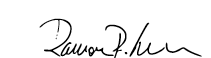
\includegraphics[width=65mm]{figs/logo/assinatura-ramon.png} \\[-4mm]
  \rule[2mm]{70mm}{0.1mm} \\
  \ramon \\[1mm]
  Coordenador do Projeto \\
}

%---------------------------------------------------------------------
\fim



 
\subsection{Abril/2015}
  \subsubsection{Minuta de reunião (16-Abril-2015)}

\begin{tabbing}
  Local \= xxx \kill
  Local \> : LEAD \\
  Data  \> : 16 de Abril de 2015 \\
  Hora  \> : 10:00
\end{tabbing}

%---------------------------------------------------------------------
\participantes{
  \elael,
  \alana,
  \gabriel,
  \julia,
  \ramon,
  \renan.
}

\begin{itemize}
  \item Aprovação da minuta.

  \item Update semanal do Projeto EMMA.
  
  \begin{itemize}
    \item \textbf{\renan.} 
		\begin{itemize}    
			 \item Reportcomp completo.
			 \item Relatório de Eletrônica
			 \item EMMA SOTA 
			
		\end{itemize}
		
		
    \item \textbf{\elael.} 
    		\begin{itemize}    
			 \item Lista de .xml
			 \item Testes executados.
			 \item Proposta Mestrado
			\end{itemize}
					
			
    \item \textbf{\gabriel.} 
    		\begin{itemize}    
			 \item Lista de .xml
			 \item Testes executados.
			 \item Proposta Mestrado
			 \item EMMA SOTA
			\end{itemize}

		 \item \textbf{\julia.} 
    		\begin{itemize}    
			 \item Desenhos de Conceito
			 \item Mestrado
			\end{itemize}

			
  \end{itemize}


  \item Agenda para a próxima reunião:
  \begin{itemize}
    \item Resultado de pesquisas individuais.
    \item Viagem Jirau Abril.
    \item Novas tarefas \& recomendações.
  \end{itemize}

\end{itemize}

\vspace{5mm}%
\parbox[t]{70mm}{
  Aprovado por: \\[5mm]
  \centering
  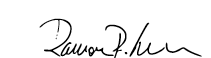
\includegraphics[width=65mm]{figs/logo/assinatura-ramon.png} \\[-4mm]
  \rule[2mm]{70mm}{0.1mm} \\
  \ramon \\[1mm]
  Coordenador do Projeto \\
}

%---------------------------------------------------------------------
\fim
  
\subsection{Maio/2015} 
  \subsubsection{Minuta de reunião (07-Maio-2015)}

\begin{tabbing}
  Local \= xxx \kill
  Local \> : LEAD \\
  Data  \> : 07 de Maio de 2015 \\
  Hora  \> : 10:00
\end{tabbing}

%---------------------------------------------------------------------
\participantes{
  \elael,
  \alana,
  \gabriel,
  \julia,
  \ramon,
  \renan.
}

\textbf{Aprovação da minuta}

\textbf{Update semanal do Projeto EMMA}
  

 \textbf{\alana.} 
	\begin{itemize}
		\item \textbf{Tarefas concluídas:}
			\begin{itemize}    
				\item Diárias e administrativo de viagem.
			\end{itemize}
		
		\item \textbf{Novas tarefas:}
			\begin{itemize} 
				\item Dados ESBR
			\end{itemize}
	\end{itemize}
  
  
\textbf{\renan.} 
	\begin{itemize}
		\item \textbf{Tarefas concluídas:}
			\begin{itemize}    
				\item Analise técnica feita durante a viagem.
			\end{itemize}
		
		\item \textbf{Novas tarefas:}
			\begin{itemize} 
				\item Formalizar análise no EMMA SOTA
				\item conceito escoltilha inferior.
			\end{itemize}
	\end{itemize}
		
\textbf{\elael.} 
	\begin{itemize}
		\item \textbf{Tarefas concluídas:}
			\begin{itemize}    
				\item Ajustes de conceito da escotilha superior.
			\end{itemize}
		
		\item \textbf{Novas tarefas:}
			\begin{itemize} 
				\item Formalizar ajustes no EMMA SOTA
				\item Relatório de viagem Latex.
			\end{itemize}
	\end{itemize}
					
			
   \textbf{\gabriel.} 
	\begin{itemize}
		\item \textbf{Tarefas concluídas:}
			\begin{itemize}    
				\item Analise técnica feita durante a viagem.
			\end{itemize}
		
		\item \textbf{Novas tarefas:}
			\begin{itemize} 
			    \item Conceito Caixa.
				\item Formalizar ajustes no EMMA SOTA
			\end{itemize}
	\end{itemize}

			



\textbf{Agenda para a próxima reunião:}
  \begin{itemize}
    \item Resultado de pesquisas individuais.
    \item Novas tarefas \& recomendações.
  \end{itemize}


\vspace{5mm}%
\parbox[t]{70mm}{
  Aprovado por: \\[5mm]
  \centering
  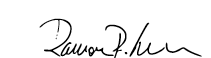
\includegraphics[width=65mm]{figs/logo/assinatura-ramon.png} \\[-4mm]
  \rule[2mm]{70mm}{0.1mm} \\
  \ramon \\[1mm]
  Coordenador do Projeto \\
}

%---------------------------------------------------------------------
\fim
  \subsubsection{Minuta de reunião (14-maio-2015)}

\begin{tabbing}
  Local \= xxx \kill
  Local \> : LEAD \\
  Data  \> : 14 de Maio de 2015 \\
  Hora  \> : 10:00
\end{tabbing}

%---------------------------------------------------------------------
\participantes{
  \elael,
  \alana,
  \gabriel,
  \julia,
  \ramon,
  \renan.
}


\textbf{Aprovação da minuta}

\textbf{Update semanal do Projeto EMMA}
  
\textbf{\renan.} 
	\begin{itemize}
		\item \textbf{Tarefas concluídas:}
			\begin{itemize}    
				\item Fez Apresentação sobre seu conceito Escotilha
     Inferior: questões gerais, pros \& cons, soluções de logística, soluções de
     robótica
			\end{itemize}
		
		\item \textbf{Novas tarefas:}
			\begin{itemize} 
				\item Começar a trabalhar com a questão de reparos de
	turbinas e como determinar a posição do manipulador em relação a pá. 
				\item Análise de Risco.
			\end{itemize}
	\end{itemize}
	
\textbf{\elael.} 
    \begin{itemize}    
		\item \textbf{Tarefas concluídas:}
			\begin{itemize}
				\item Questões comuns do problema.
				\item Consolidar possiveis soluções 
			\end{itemize}
			
		\item \textbf{Novas tarefas:}
			\begin{itemize} 
				\item Calcular base articulada.
				\item Verificar payload.			
			\end{itemize}
	\end{itemize}
	
\textbf{\gabriel.} 
	\begin{itemize}
		\item \textbf{Tarefas concluídas:}
			\begin{itemize}    
				\item Questões comuns do problema.
				\item Consolidar possiveis soluções 
			\end{itemize}
		\item \textbf{Novas tarefas:}
			\begin{itemize}
				\item Calcular base articulada.
				\item Verificar payload.		
			\end{itemize}
	\end{itemize}
	
\textbf{\julia.} 
	\begin{itemize}
		\item \textbf{Tarefas concluídas:}
			\begin{itemize}    
				\item Administrativo Relátorios e Notas.
				\item Tradução para SOTA.
				\item Entrevista com possíveis orientadores.
			\end{itemize}
		\item \textbf{Novas tarefas:}
			\begin{itemize}
				\item Dados ESBR.
				\item Revisão de Proposta.		
			\end{itemize}
	\end{itemize}

%   \item Problemas em aberto:
%   \begin{itemize}
%     \item Procedimento de compras e medidas para as instalações finais do
%     laboratório.
%     \item Opções para a comprar de software, Adobe/ Solid Works/ Live
%     Meeting/Bibliografia
%     \item Fechar orçamento Inventário.
%     \item Criar log para documentar problemas de ROCK/ criar um forum para
%     colaboração (?!)
%     \item Dropbox para compartilhamento de arquivos.
%     \item Viagem ESB/Relatório:
%   \end{itemize}
\textbf{Agenda para a próxima reunião:}
  \begin{itemize}
    \item Resultado de pesquisas individuais.
    \item Viagem Jirau Abril.
    \item Novas tarefas \& recomendações.
  \end{itemize}

\vspace{5mm}%
\parbox[t]{70mm}{
  Aprovado por: \\[5mm]
  \centering
  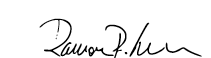
\includegraphics[width=65mm]{figs/logo/assinatura-ramon.png} \\[-4mm]
  \rule[2mm]{70mm}{0.1mm} \\
  \ramon \\[1mm]
  Coordenador do Projeto \\
}

%---------------------------------------------------------------------
\fim
  \subsubsection{Minuta de reunião (21-Maio-2015)}

\begin{tabbing}
  Local \= xxx \kill
  Local \> : LEAD \\
  Data  \> : 21 de Maio de 2015 \\
  Hora  \> : 10:00
\end{tabbing}

%---------------------------------------------------------------------
\participantes{
  \elael,
  \alana,
  \gabriel,
  \julia,
  \ramon,
  \renan.
}

  
\begin{itemize}
  \item Aprovação da minuta.

  \item Update semanal do Projeto EMMA.
  
  
    \item \textbf{\renan.} 
		\begin{itemize}    
			 \item Apresentação conceito Escotilha Inferior
			 \item Correções EMMA SOTA 
			
		\end{itemize}
		
		
    \item \textbf{\elael.} 
    		\begin{itemize}    
			 \item Apresentação conceito Escotilha Superior. 
			 \item Correções EMMA SOTA 
			\end{itemize}
					
			
    \item \textbf{\gabriel.} 
    		\begin{itemize}    
		 \item Apresentação conceito Caixa. 
		 \item Correções EMMA SOTA. 
			\end{itemize}

		 \item \textbf{\julia.} 
    		\begin{itemize}    
			 \item Relatórios ESBR
			 \item PR EMMA/Projeto no Site
			 \item Livro de Atas
		
			\end{itemize}


  \item Agenda para a próxima reunião:
  \begin{itemize}
    \item Resultado de pesquisas individuais.
    \item Novas tarefas \& recomendações.
  \end{itemize}

\end{itemize}

\vspace{5mm}%
\parbox[t]{70mm}{
  Aprovado por: \\[5mm]
  \centering
  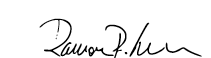
\includegraphics[width=65mm]{figs/logo/assinatura-ramon.png} \\[-4mm]
  \rule[2mm]{70mm}{0.1mm} \\
  \ramon \\[1mm]
  Coordenador do Projeto \\
}

%---------------------------------------------------------------------
\fim
  %---------------------------------------------------------------------
\subsubsection{Minuta de reunião (28-maio-2015)}

\begin{tabbing}
  Local \= xxx \kill
  Local \> : LEAD \\
  Data  \> : 28 de Maio de 2015 \\
  Hora  \> : 10:00
\end{tabbing}

%---------------------------------------------------------------------
\participantes{
  \elael,
  \gabriel,
  \julia,
  \patrick,
  \alana,
  \ramon,
  \renan.
}

\textbf{Aprovação da minuta}

\textbf{Update semanal do Projeto EMMA}
  
\textbf{\renan.} 
	\begin{itemize}
		\item \textbf{Tarefas concluídas:}
			\begin{itemize}    
				\item Ajustes de conceito da escotilha inferior.
			\end{itemize}
		
		\item \textbf{Novas tarefas:}
			\begin{itemize} 
				\item Formalizar ajustes no EMMA SOTA
			\end{itemize}
	\end{itemize}
	
\textbf{\elael.} 
    \begin{itemize}    
		\item \textbf{Tarefas concluídas:}
			\begin{itemize}
				\item Análise de torc e vibração.
				\item Explorou possibilidades para menosr vibração.
				\item Possibilidades relacionadas ao tamanho de braço do robô
			\end{itemize}
			
		\item \textbf{Novas tarefas:}
			\begin{itemize} 
				\item ver com Ramon se será necessário o uso de um 'demper'ou não.
				\item Ver a menos velocidade na qual a base permitirá a continuidade do
				processo de coating.
				\item Frmalizar alterações no SOTA.
			\end{itemize}
	\end{itemize}
	
\textbf{\gabriel.} 
	\begin{itemize}
		\item \textbf{Tarefas concluídas:}
			\begin{itemize}    
				\item Problemas relacionados ao ambiente da unidade geradora.
				\item Ë preciso entender como a curvatura do ambiente pode alterar a
				estabilidade do braço.
			\end{itemize}
		\item \textbf{Novas tarefas:}
			\begin{itemize}
				\item Parafusos nmmagnéticos: qual teria de ser o peso para segurar a base.
				Efeitos colaterais de agua, pressão e deformidade do ambiente.
				\item Frmalizar alterações no SOTA.		
			\end{itemize}
	\end{itemize}
	
\textbf{\julia.} 
	\begin{itemize}
		\item \textbf{Tarefas concluídas:}
			\begin{itemize}    
				\item Administrativo Relátorios e Notas
				\item Mestrado 
			\end{itemize}
		\item \textbf{Novas tarefas:}
			\begin{itemize}
				\item Apresentação EMMA, formalizar o conteúdo do projeto de
				forma clara para divulgação e explicação do projeto.
				\item Vídeo EMMA Aevo.
			\end{itemize}
	\end{itemize}
%   \item Problemas em aberto:
%   \begin{itemize}
%     \item Procedimento de compras e medidas para as instalações finais do
%     laboratório.
%     \item Opções para a comprar de software, Adobe/ Solid Works/ Live
%     Meeting/Bibliografia
%     \item Fechar orçamento Inventário.
%     \item Criar log para documentar problemas de ROCK/ criar um forum para
%     colaboração (?!)
%     \item Dropbox para compartilhamento de arquivos.
%     \item Viagem ESB/Relatório:
%   \end{itemize}

\textbf{Agenda para a próxima reunião:}
	\begin{itemize}
		\item Resultado de pesquisas individuais.
	    \item Viagem Jirau Abril.
	    \item Novas tarefas \& recomendações.
	\end{itemize}


\vspace{5mm}%
\parbox[t]{70mm}{
  Aprovado por: \\[5mm]
  \centering
  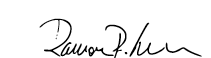
\includegraphics[width=65mm]{figs/logo/assinatura-ramon.png} \\[-4mm]
  \rule[2mm]{70mm}{0.1mm} \\
  \ramon \\[1mm]
  Coordenador do Projeto \\
}

%---------------------------------------------------------------------
\fim


 
% \newpage%
% \subsection{Abril/2015}
%    \input{minuta-de-reuniao(16-nov-2013)}
%   %---------------------------------------------------------------------
\subsubsection{Minuta de reuni�o (06-nov-2013)}

\begin{tabbing}
  Local \= xxx \kill
  Local \> : LEAD \\
  Data  \> : 06 de Novembro de 2013 \\
  Hora  \> : 11:00
\end{tabbing}

%---------------------------------------------------------------------
\participantes{
  \antonio,
  \gizele (via telefone),
  \julia,
  \patrick,
  \ramon.
}

\pauta{Reuni�o com Antonio da COPPETEC para discutir procedimentos de pagamentos do projeto com a ESBR.}

\begin{itemize}
  \item Abertura. A reuni�o do Projeto ROSA foi convocada por \ramon.

  %\item Aprova��o da minuta da reuni�o anterior.

  \item Itens em aberto:
  \begin{itemize}
    \item Emiss�o de nota para pagamento da parcela do projeto. (\textbf{Ant�nio})

    \item Gisele: Pagamento da parcela. \\
        O valor dessa primeira parcela, procedimentos, o que � preciso para efetuar o pagamento e o prazo para tal. (\textbf{Definir})

    \item Necessidade de um of�cio mensal para os bolsistas, assim como uma nota que discrimine do valor incluso da taxa administrativa da nota fiscal para o controle. (\textbf{Ant�nio})

    \item Presta��o de contas final. Segundo os procedimentos de PID da ANEEL, � necess�rio um relat�rio final de projeto discriminando qualquer altera��o da proposta original com toda a presta��o de contas. A Gizele fornecer� uma planilha para a COPPETEC nos moldes da ESBR para que coincida com o cronograma estabelecido. (\textbf{Ant�nio})

    \item A COPPETEC faz pagamentos sempre 5, 15 e 25 de cada m�s. Temos que mandar planilha essa semana para receber dia 25.

    \item Mandar formul�rio com os contratados CLT RH COPPETEC. (\textbf{Gerente Gabriel})

    \item Pedir formul�rios para infraestrutura do Laborat�rio, CLT e contra��o de terceiros. (\textbf{Fabiana COPPETEC})

    \item Viagem: COPPETEC permite di�ria nacional de R\$\,300,00 e internacional de US\$\,350,00. Nossa viagem j� foi paga pela ESBR e depois ser� descontada em parcela futura. \\
        Contato para passagens: Word Turismo.

    \item Indica��o da COPPETEC para Secret�ria Administrativa.
  \end{itemize}

  \item Pauta para a pr�xima reuni�o: N�o definida.

\end{itemize}

\vspace{10mm}%
\parbox[t]{70mm}{
  Aprovado por: \\[5mm]
  \centering
  %\includegraphics[bb=1 1 1238 299,width=65mm]{../assinatura/assinatura-digital.jpg} \\[-4mm]
  \includegraphics[width=65mm]{../assinatura/assinatura-digital.jpg} \\[-4mm]
  \rule[2mm]{70mm}{0.1mm} \\
  \ramon \\[1mm]
  Coordenador do Projeto \\
}

%---------------------------------------------------------------------
\fim

%   %---------------------------------------------------------------------
\subsubsection{Minuta de reuni�o (11-nov-2013)}

\begin{tabbing}
  Local \= xxx \kill
  Local \> : Usina Hidrel�trica de Jirau (UHE) \\
  Data  \> : 11 de Novembro de 2013 \\
  Hora  \> : 09:00
\end{tabbing}

%---------------------------------------------------------------------
\participantes{
  \jacoud,
  \breno,
  \gizele,
  \julia,
  \patrick,
  \ramonC,
  \ramon.
}

\pauta{Reuni�o de abertura do Projeto ROSA (PD-6631-0002/2013).}

\begin{itemize}
  %\item Abertura. A reuni�o do Projeto ROSA foi convocada por \ramon.

  \item Apresenta��o de nossa proposta e pontos de discuss�o. \\
      Confirma��o dos erros atuais da opera��o, discuss�o em tornos de todos os aspectos do processo de inser��o e remo��o de \emph{stoplogs}.

  \item Problema de engate, de encaixe das garras, necessidade de nivela��o. Sensores podem ajudar a determinar inclina��o e os detritos que interferem no processo.

  \item Ac�mulo de detritos nas garras e na lateral do \emph{stoplog} n�o permitem a visualiza��o.

  \item Falta controle de inclina��o dos \emph{stoplogs}. Ainda n�o e poss�vel determinar o desn�vel com precis�o.

  \item O operador tem liberdade para manejar o \emph{stoplog} no guindaste por�m a opera��o � mec�nica, feita por tentativa e erro, necessitando de um mapeamento mais preciso em que possamos nos basear para construir o sistema operacional.

  \item O processo tem apenas um display digital com o peso levantado na estrutura do guindaste.

  \item Os sensores de contato precisam ter uma prote��o robusta afim de sobreviver ao tipo de ambiente.

  \item � necess�ria uma interface com operador para mapeamento do poss�vel sistema operacional e op��es do sistema atual.

  \item Proposta:
  \begin{itemize}
    \item Adicionar eletr�nica na viga pescadora e sensores de for�a/contato nas garras para determinar engate correto. O operador precisa visualizar ao m�ximo o ambiente a fim de operar o \emph{stoplog} com sucesso.

    \item Instalar c�meras que permitam ver a garra em si. Um sonar 3D far� o mapeamento do fundo para saber o tamanho e volume do que estiver abaixo da viga pescadora.

    \item Pesquisa do que j� existe em termos de interface. Conhecer/entender a integra��o gr�fica com o sistema do Rock. (\textbf{Julia e Rafael}) \\
  \end{itemize}

  \item A segunda parte da reuni�o foi coordenada por Gizele. Ela abordou quest�es administrativas.

  \item Sobre o relat�rio mensal:
  \begin{itemize}

    \item Modelos de notas fiscais assim como os modelos do relat�rio mensal e quadrimestral.

    \item Per�odo, coordenador, gerente (assinaturas)

    \item Solicita��es de pagamento, comprovantes de atua��o /controle de ponto para adicionar ao processo de pagamento.

    \item Relat�rio fotogr�fico das atividades realizadas

    \item Equipe t�cnica de trabalho discriminado.

    \item Planos de trabalho (tarefas executadas, atas de reuni�o)
  \end{itemize}

  \item Sobre o relat�rio quadrimestral:
  \begin{itemize}
    \item Per�odo, datas de emiss�o.
    \item Objetivo, teses e disserta��es.
    \item Pesquisadores e subprojetos.
    \item Plano de trabalho atualizado (tarefas executadas, timeline).
    \item Outorga de pesquisadores (termo de conduta dos pesquisadores).
    \item Atividades previstas no per�odo de 4 meses (resumo dos relat�rios mensais durante 4 meses).
    \item Providenciar MS Project para o projeto.
    \item Di�rias: valores limites, reembolso x di�rias (fazer pedidos ao menos 5 dias antes).
    \item Relat�rio de viagem, objetivo, resumo, fracasso x sucesso e valor total.
    \item Solicita��o de loca��o de ve�culos
    \item Controle de staff: Termo de outorga e termo de vig�ncia
  \end{itemize}

  \item A Fazer:
  \begin{itemize}
    \item Passar o projeto para MS Project (\textbf{Patrick}).
    \item Tabela oficial de di�rias (solicita��es de di�rias x reembolso).
    \item Criar relat�rio mensal equivalente a Outubro, destacando a mobiliza��o de estrutura.
    \item Atualizar atas de acordo com regras do projeto (aprovadas por Ramon e tirar 'enviada por'.)
    \item Estabelecer regras de trabalho com staff, sistemas de ponto e hor�rios.

    \item Em rela��o �s folhas de ponto:
    \begin{itemize}
      \item	Verificar quem � o respons�vel pelo preenchimento do modelo de folhas de ponto mensal. (\textbf{Ramon})
      \item	Verificar com a COPPETEC como � feito em outros projetos.
      \item	Template para o preenchimento da tabela de pontos de cada funcion�rio a ser enviada no fim do m�s.
      \item	Periodicidade: Mensal.
    \end{itemize}

    \item Formul�rios REFP:
    \begin{itemize}
      \item	Verificar com Ant�nio como � feito o preenchimentos do formul�rio REFP
      \item	Informa��o aos fornecedores. Verificar com Antonio se esta tudo OK para emiss�o de notas.
      \item	Periodicidade: Quadrimestral.
    \end{itemize}

    \item Modelo de of�cio de solicita��o de pagamento de bolsistas do projeto P\&D:
    \begin{itemize}
      \item	Reuni�o com Antonio para verificar se ele esta ciente de tal procedimento.
      \item	Tem que ser preenchido sempre que solicitada alguma verba.
    \end{itemize}

    \item Modelo de recibo de bolsista:
    \begin{itemize}
      \item	Verificar m�todo utilizado pela UFRJ e informar � Gizele o procedimento.
      \item	Todas as bolsas entram em um tabela �nica.
    \end{itemize}

    \item Termo de outorga:
    \begin{itemize}
      \item	Verificar se modelo COPPETEC est'a de acordo.
       \item As informa��es necess�rias s�o; nome do projeto, n�mero do contrato e n�mero perante a ANEEL.
    \end{itemize}

    \item Presta��o de contas:
    \begin{itemize}
      \item	Relat�rio de viagem.
      \item	Passar por Ant�nio para saber se est� de acordo com o modelo COPPETEC.
    \end{itemize}

    \item Modelo de Relat�rio Mensal:
    \begin{itemize}
      \item	Objetivos.
      \item	Aspectos relevantes.
      \item	Relat�rio fotogr�fico.
      \item	Atividades previstas.
      \item	Equipe t�cnica de trabalho.
    \end{itemize}
  \end{itemize}

%  \item Pauta para a pr�xima reuni�o: N�o definida.

\end{itemize}

\vspace{10mm}%
\parbox[t]{70mm}{
  Aprovado por: \\[5mm]
  \centering
  %\includegraphics[bb=1 1 1238 299,width=65mm]{../assinatura/assinatura-digital.jpg} \\[-4mm]
  \includegraphics[width=65mm]{../assinatura/assinatura-digital.jpg} \\[-4mm]
  \rule[2mm]{70mm}{0.1mm} \\
  \ramon \\[1mm]
  Coordenador do Projeto \\
}

%---------------------------------------------------------------------
\fim

%   %---------------------------------------------------------------------
\subsubsection{Minuta de reuni�o (18-nov-2013)}

\begin{tabbing}
  Local \= xxx \kill
  Local \> : LEAD \\
  Data  \> : 18 de Novembro de 2013 \\
  Hora  \> : 14:00
\end{tabbing}

%---------------------------------------------------------------------
\participantes{
  \jacoud,
  \elael,
  \gabriel,
  \julia,
  \patrick,
  \rafael,
  \ramon,
  \renan.
}

\pauta{Relat�rio de viagem e acompanhamento das atividades.}

\begin{itemize}
  \item Abertura. A reuni�o do Projeto ROSA foi convocada por \ramon.

  \item Aprova��o da minuta da reuni�o anterior.

  \item Apresenta��o de relat�rio de viagem para os presentes. \\
      Descri��o da opera��o de inser��o e retirada de \emph{stoplog} presenciada pela equipe que viajou � Porto Velho. Detalhes do processo, fotos e \emph{brainstorming} de possibilidades para a solu��o que vamos implementar.

  \item Update de reuni�o com Sylvain e novas tarefas.

  \item Novas tarefas para o grupo de software.
  \begin{itemize}
    \item \textbf{\gabriel.} Estudar t�cnicas de representa��o de estruturas tridimensional. Integrar a biblioteca do OctoMap ao Rock e fazer funcionar.

    \item \textbf{\elael.} Simular um sonar. Testar laser scanner para saber se a reconstru��o da estrutura � feita corretamente no OctoMap.

    \item \textbf{\rafael.} Estudar a reconstru��o de estruturas. Fazer a simula��o e buscar o percentual de espa�o ocupado pelo sonar.
  \end{itemize}

  \item Novas tarefas para o grupo de pot�ncia.
  \begin{itemize}
    \item \textbf{\andre.} Pesquisar sistemas de pot�ncia e umbilicais para o projeto. Enviar o  resultado da pesquisa para o Patrick. Complemento da pesquisa: Equipamento de terra necess�rio para os cabos.

    \item \textbf{\renan.} Pesquisar sensores.
  \end{itemize}

  \item Novas tarefas para o grupo de design.
  \begin{itemize}
    \item \textbf{\julia.} Pesquisar a integra��o de interfaces no Rock. Fazer pesquisa bibliogr�fica. Estudo b�sico de integra��o do Rock (parceria com programa��o).
  \end{itemize}

%  \item Pauta para a pr�xima reuni�o: N�o definida.

\end{itemize}

\vspace{10mm}%
\parbox[t]{70mm}{
  Aprovado por: \\[5mm]
  \centering
  %\includegraphics[bb=1 1 1238 299,width=65mm]{../assinatura/assinatura-digital.jpg} \\[-4mm]
  \includegraphics[width=65mm]{../assinatura/assinatura-digital.jpg} \\[-4mm]
  \rule[2mm]{70mm}{0.1mm} \\
  \ramon \\[1mm]
  Coordenador do Projeto \\
}

%---------------------------------------------------------------------
\fim

%   %---------------------------------------------------------------------
\subsubsection{Minuta de reuni�o (25-nov-2013)}

\begin{tabbing}
  Local \= xxx \kill
  Local \> : LEAD \\
  Data  \> : 18 de Novembro de 2013 \\
  Hora  \> : 09:00
\end{tabbing}

%---------------------------------------------------------------------
\participantes{
  \jacoud,
  \andre,
  \elael,
  \gabriel,
  \julia,
  \patrick,
  \rafael,
  \ramon,
  \renan,
  \sylvain.
}

\pauta{Acompanhamento das atividades.}

\begin{itemize}
  \item Abertura. A reuni�o do Projeto ROSA foi convocada por \ramon.

  \item Aprova��o da minuta da reuni�o anterior.

  \item O grupo de software resumiu suas atividades.
  \begin{itemize}
    \item \textbf{\gabriel.} Deu continuidade ao trabalho no Rock Robotics, explorando as formas de usar Octomap. Enviou d�vidas para Sylvain e aguarda feedback. Estudou artigos e separou bibliografia no Mendeley. \\

    \item \textbf{\rafael.} Pesquisa com simula��o e espa�o ocupado pelo sonar. Depois de reuni�o individual com Patrick ter� acesso a data (DFKI) que o ajudar� com as simula��es. Tamb�m encontrou artigos para refer�ncia. \\

    \item \textbf{\elael.} Buscando a melhor forma de testar scanner para saber se a reconstru��o da estrutura � feita corretamente no OctoMap. \\
  \end{itemize}

  \item O grupo de pot�ncia resumiu suas atividades.
  \begin{itemize}
    \item \textbf{\andre.} Pesquisou Sistemas de Pot�ncia e umbilicais para o projeto. Complemento da pesquisa: Equipamento de terra necess�rio para os cabos. \\

    \item \textbf{\renan.} Fazendo an�lise para fluxograma. \\
  \end{itemize}

  \item O grupo de design resumiu suas atividades.
  \begin{itemize}
    \item \textbf{\julia.} Pesquisou sobre QT e integra��o de interfaces no Rock. Fez pesquisa bibliogr�fica. O tema de Mestrado est� em aberto. Estado b�sico de integra��o do Rock (parceria com programa��o) estabelecer processo. \\
  \end{itemize}

%  \item Pauta para a pr�xima reuni�o: N�o definida.

\end{itemize}

\vspace{10mm}%
\parbox[t]{70mm}{
  Aprovado por: \\[5mm]
  \centering
  %\includegraphics[bb=1 1 1238 299,width=65mm]{../assinatura/assinatura-digital.jpg} \\[-4mm]
  \includegraphics[width=65mm]{../assinatura/assinatura-digital.jpg} \\[-4mm]
  \rule[2mm]{70mm}{0.1mm} \\
  \ramon \\[1mm]
  Coordenador do Projeto \\
}

%---------------------------------------------------------------------
\fim


% \newpage%
% \subsection{Dezembro/2013}
%   %---------------------------------------------------------------------
\subsubsection{Minuta de reuni�o (02-dez-2013)}

\begin{tabbing}
  Local \= xxx \kill
  Local \> : LEAD \\
  Data  \> : 02 de Dezembro de 2013 \\
  Hora  \> : 10:00
\end{tabbing}

%---------------------------------------------------------------------
\participantes{
  \jacoud,
  \andre,
  \elael,
  \gabriel,
  \julia,
  \rafael,
  \ramon,
  \renan.
}

\pauta{Acompanhamento das atividades.}

\begin{itemize}
  \item Abertura. A reuni�o do Projeto ROSA foi convocada por \ramon.

  \item Aprova��o da minuta da reuni�o anterior.

  \item Em aberto:
  \begin{itemize}
    \item Software de ScrumDo.
    \item Forum de Sonares dia 10 aqui na UFRJ.
    \item Ver Mendeley vers�o times (usado no DFKI).
    \item Substituto para Rafael. Encontrar candidato. \\
  \end{itemize}

  \item Tarefas para o coordenador:
  \begin{itemize}
    \item Proposta CIR to UFRJ. Conferir e assinar.
    \item Escopo do Projeto. Conferir e assinar.
    \item Relat�rio de usabilidade. Conferir e assinar.
    \item Assinar requerimentos para aquisi��o: laptops LENOVO, sensor, sonar e encoder. \\
  \end{itemize}

  \item Tarefas para o Alessandro:
  \begin{itemize}
    \item Feedback de relat�rios de usabilidade e escopo do projeto.
    \item Software de Scrum. Ser� o respons�vel por coordenar nosso scrum e quadro de tarefas.
    \item Viabilizar ScrumDo para todo LEAD (conversar com Lucas) afim que tenhamos controle de cada participante em todos os projetos vigentes.
    \item Criar quadro na nossa sala para visualizar tarefas do Projeto ROSA. \\
  \end{itemize}

  \item Atividades do Sylvain:
  \begin{itemize}
    \item Conversou com o time de software, estamos na mesma pagina. Mencionou a troca de Sonar, confirmar com Patrick se o Sonar que esta no relat�rio � o correto. \\
  \end{itemize}

  \item Tarefas para o grupo de design (\textbf{\julia}.
  \begin{itemize}
    \item Relat�rio de usabilidade.
    \item Escopo do projeto traduzido.
    \item Entregar requerimentos de compras para sonar, sensor e codificador.
    \item Pedir a Ant�nio status do nosso do or�amento e fazer um RAP.
    \item Providenciar junto � COPPETEC o seguro de vida da equipe.
    \item Fazer preparativos para a viagem de Renan para Alemanha.
    \item Adicionar folhas de ponto dos CLT's assinadas por todos. Escanear e adicionar ao relat�rio.
    \item Marcar com Patrick a reuni�o para discutir o conceito. \\
  \end{itemize}

  \item Atividades do grupo de software.
  \begin{itemize}
    \item \textbf{\gabriel.} Octomap integrado ao ROCK, precisa de update. Trabalhando no OctoViz. J� obteve feedback do Sylvain. Para essa semana vai continuar no Octoviz. Achou um artigo relativo ao trabalho. Come�ou a usar o GUIT. \\

    \item \textbf{\elael.} Trabalhou/pesquisou um tipo de simula��o mais realista do Sonar. Filtrou alguns artigos mas a maioria est� mais voltada para o chamado Sonar Lateral (submarinos e foguetes). Instalou GUIT. Implementa��o da renderiza��o off screen, pelo buffer, conseguindo extrair dela o Z-Buffer. Encontrou problemas com a configura��o com rela��o ao tamanho do contexto utilizado para gerar o pixel buffer, parece functional mas talvez esteja gastando processamento e c�digo a toa. Problema de documenta��o com o OSG.  Esse semana vai trabalhar em passar o c�digo do OSG para o Ubuntu afim de criar o driver Rock que vai ser utilizado para criar o componente do simulador. \\
  \end{itemize}

  \item Atividades do grupo de pot�ncia.
  \begin{itemize}
    \item \textbf{\andre.} Pelo que pesquisou, descobriu que h� possibilidade de pedir o carretel mas n�o necessariamente ordenar o cabo junto. Poder�amos ordenar um cabo separado configurado para o nosso projeto. O �nico problema � que esses carreteis t�m contato girante (slip ring) que n�o � compat�vel com fibra �tica. Vai mandar email para o Patrick detalhando. \\

    \item \textbf{\renan.} Acabou a pesquisa de mercado dos sensors e compilou os sensors que poderiam ser usados no projeto de acordo com especifica��o (Tabela Excel). Tamb�m pesquisou empresas que podem fazer o encapsulamento e empresas que j� fazem a eletr�nica embarcada e o housing. \\
  \end{itemize}

%  \item Pauta para a pr�xima reuni�o: N�o definida.

\end{itemize}

\vspace{10mm}%
\parbox[t]{70mm}{
  Aprovado por: \\[5mm]
  \centering
  %\includegraphics[bb=1 1 1238 299,width=65mm]{../assinatura/assinatura-digital.jpg} \\[-4mm]
  \includegraphics[width=65mm]{../assinatura/assinatura-digital.jpg} \\[-4mm]
  \rule[2mm]{70mm}{0.1mm} \\
  \ramon \\[1mm]
  Coordenador do Projeto \\
}

%---------------------------------------------------------------------
\fim

%   %---------------------------------------------------------------------
\subsubsection{Minuta de reuni�o (09-dez-2013)}

\begin{tabbing}
  Local \= xxx \kill
  Local \> : LEAD \\
  Data  \> : 09 de Dezembro de 2013 \\
  Hora  \> : 10:00
\end{tabbing}

%---------------------------------------------------------------------
\participantes{
  \jacoud,
  \andre,
  \elael,
  \gabriel,
  \julia,
  \ramon,
  \renan.
}

\pauta{Acompanhamento das atividades.}

\begin{itemize}
  \item Abertura. A reuni�o do Projeto ROSA foi convocada por \ramon.

  \item Aprova��o da minuta da reuni�o anterior.

  \item Em aberto:
  \begin{itemize}
    \item Criar of�cios para obter as rubricas (Ant�nio e Gizele).
    \item Seguro de Sa�de.
    \item Substituto para Rafael, encontrar candidato.
    \item Reuni�o para discutir conceito. Agendar com os grupos para o dia 16/12. Trazer anota��es. \\
  \end{itemize}

  \item Tarefas para o coordenador.
  \begin{itemize}
    \item Requerimentos para aquisi��o: laptops LENOVO, sensor, sonar e encoder, nacionais e importados.
    \item Of�cios para obter notas de projeto. \\
  \end{itemize}

  \item Tarefas para Jacoud.
  \begin{itemize}
    \item Software de Scrum: ser� o respons�vel por coordenar nosso scrum e quadro de tarefas.
    \item Viabilizar ScrumDo para todo LEAD afim de que tenhamos controle de cada participante em todos os projetos vigentes.
    \item Criar quadro na nossa sala para visualizar tarefas do Projeto ROSA. \\
  \end{itemize}

  \item Sylvain.
  \begin{itemize}
    \item N�o participar� da reuni�o �s 10:00. Ele far� uma reuni�o posterior com o grupo de software durante a tarde. \\
  \end{itemize}

  \item Grupo de design (Julia)
  \begin{itemize}
    \item Entregar requerimento de compra de sonar (ESBR), sensor e codificador.
    \item Coordenar com Ant�nio e Gizele a quest�o das rubricas.
    \item COPPETEC: Seguro de vida da equipe.
    \item Contrato de transfer�ncia para Alemanha do Renan finalizado. \\
  \end{itemize}

  \item Time Software
  \begin{itemize}
    \item \textbf{\gabriel.} Estudou Octoviz para entender funcionamento. Construiu a base do plugin 3D e esta em fase de teste. \\

    \item \textbf{\elael.} Acabou de transcrever o c�digo com a ressalva de que o pixel buffer n�o est� funcionando da mesma forma que funcionava no Windows (pode ser sintaxe ou placa de v�deo). Fez os testes de precis�o do z-buffer e encontrou um problema: funcionamento normal mas a partir de 25 unidades de dist�ncia ele d� o mesmo resultado. Seguindo recomenda��es do Sylvain, vai postar perguntas no forum online. \\
  \end{itemize}

  \item Grupo de pot�ncia
  \begin{itemize}
    \item \textbf{\andre.} Levantou pontos necess�rios para usar o cabo de fibra �tica. J� mandou para o Patrick. Preparar abstract para reuni�o sobre conceito. \\

    \item \textbf{\renan.} Pesquisa sobre sonares e sobre Pan \& Tilt. Conversou com um representante da Kongsberg e ele deu a possibilidade deles gerarem um solu��o espec�fica para o nosso caso. A ser combinado na reuni�o de conceito. \\
  \end{itemize}

%  \item Pauta para a pr�xima reuni�o: N�o definida.

\end{itemize}

\vspace{10mm}%
\parbox[t]{70mm}{
  Aprovado por: \\[5mm]
  \centering
  %\includegraphics[bb=1 1 1238 299,width=65mm]{../assinatura/assinatura-digital.jpg} \\[-4mm]
  \includegraphics[width=65mm]{../assinatura/assinatura-digital.jpg} \\[-4mm]
  \rule[2mm]{70mm}{0.1mm} \\
  \ramon \\[1mm]
  Coordenador do Projeto \\
}

%---------------------------------------------------------------------
\fim

%   %---------------------------------------------------------------------
\subsubsection{Minuta de reuni�o (17-dez-2013)}

\begin{tabbing}
  Local \= xxx \kill
  Local \> : LEAD \\
  Data  \> : 17 de Dezembro de 2013 \\
  Hora  \> : 10:00
\end{tabbing}

%---------------------------------------------------------------------
\participantes{
  \jacoud,
  \andre,
  \elael,
  \gabriel,
  \julia,
  \ramon,
  \renan.
}

\pauta{Acompanhamento das atividades.}

\begin{itemize}
  \item Abertura. A reuni�o do Projeto ROSA foi convocada por \ramon.

  \item Aprova��o da minuta da reuni�o anterior.

  \item Em aberto:
  \begin{itemize}
    \item Assinar of�cios para obter as rubricas.
    \item Ajuste no seguro de vida.
    \item Encontrar substituto para o Rafael.
    \item Encontrar/contratar engenheiro mec�nico.
    \item Requerimentos para aquisi��o de laptops LENOVO, sensor, sonar e encoder, nacionais e importados.
    \item Entregar requerimentos de compras para sonar (ESBR), sensor e codificador
    \item Contrato de transfer�ncia para Alemanha do Renan finalizado.
  \end{itemize}

  \item Tarefas para o Jacoud:
  \begin{itemize}
    \item Coordenar quest�es e tarefas para \andre.
    \item Introduzir ScrumDo como refer�ncia para nosso projeto.
  \end{itemize}

  \item Sylvain:
  \begin{itemize}
    \item N�o participar� da reuni�o pois n�o temos internet.
  \end{itemize}

  \item Grupo de design:
  \begin{itemize}
  \item \textbf{\julia.} Coordenou entrega de Relat�rio Mensal, Relat�rio de Usabilidade e de toda documenta��o para a ESBR. Quest�es administrativas em andamento. Fez apresenta��o de prot�tipos e testes que podem ser usados no projeto.
  \end{itemize}

  \item Grupo de software:
  \begin{itemize}
    \item \textbf{\gabriel.} Est� trabalhando no que foi recomendado pelo Sylvain. Construiu um componente Orogen para fazer um tipo opaco do Octomap/Octree que se comunica com o Plug-in. Fez apresenta��o do Octoviz para explicar no que tem trabalhado.

    \item \textbf{\elael.} Fechou o driver em ROCK com a ressalva de que o pixel buffer ainda esta inst�vel. Corrigiu o problema do Z-Buffer. Pr�ximo passo � avan�ar no component ROCK.
  \end{itemize}

  \item Grupo de pot�ncia:
  \begin{itemize}
    \item \textbf{\andre.} Precisa de direcionamento maior para que possa continuar na pesquisa. Aguarda o feedback.  Alessandro vai coordenar algumas tarefas para direcionar essa pesquisa.

    \item \textbf{\renan.} Aguardando o feedback do Patrick a respeito do Sonar e da proforma do Sensor indutivo (importado). Marcou reuni�o com o pessoal da Tritec. Fez apresenta��o com um resumo do que j� pesquisou, � o que est� em aberto. Tamb�m fez um sketch sobre a eletr�nica geral do projeto (evolu��o de acordo com as mudan�as) assim como se dedicou ao power supply. Conversou com Igor (Projeto DORIS) sobre a possibilidade de usar uma bateria embarcada ao inv�s de um umbilical.
  \end{itemize}

%  \item Pauta para a pr�xima reuni�o: N�o definida.

\end{itemize}

\vspace{10mm}%
\parbox[t]{70mm}{
  Aprovado por: \\[5mm]
  \centering
  %\includegraphics[bb=1 1 1238 299,width=65mm]{../assinatura/assinatura-digital.jpg} \\[-4mm]
  \includegraphics[width=65mm]{../assinatura/assinatura-digital.jpg} \\[-4mm]
  \rule[2mm]{70mm}{0.1mm} \\
  \ramon \\[1mm]
  Coordenador do Projeto \\
}

%---------------------------------------------------------------------
\fim

% 
% \newpage%
% \subsection{Janeiro/2014}
%   %---------------------------------------------------------------------
\subsubsection{Minuta de reuni�o (06-jan-2014)}

\begin{tabbing}
  Local \= xxx \kill
  Local \> : LEAD \\
  Data  \> : 06 de Janeiro de 2014 \\
  Hora  \> : 10:00
\end{tabbing}

%---------------------------------------------------------------------
\participantes{
  \jacoud,
  \andre,
  \elael,
  \gabriel,
  \julia,
  \ramon,
  \renan.
}

\pauta{Acompanhamento das atividades.}

\begin{itemize}
  \item Abertura. A reuni�o do Projeto ROSA foi convocada por \ramon.

  \item Aprova��o da minuta da reuni�o anterior.

  \item Em aberto:
  \begin{itemize}
    \item Finalizar of�cios.
    \item Seguro de vida finalizado.
    \item Of�cio \#4: solicita��o de recursos para viagem dos CLT's para Alemanha.
    \item Temas de mestrado.
    \item Of�cios \#4, \#5 e \#6. Rafael tem of�cio espec�fico uma vez que vai como Mestrando. Fechar com RH os detalhes do contrato.)
  \end{itemize}

  \item Jacoud:
  \begin{itemize}
    \item Auxiliar \andre na defini��o do tema de mestrado e prepara abstract.
  \end{itemize}

  \item Grupo de design
  \begin{itemize}
    \item \textbf{\julia.} Finalizar entrega de Relat�rio Mensal. Quest�es administrativas em andamento. Preparar prot�tipo da interface do operador para executar teste em Fevereiro.
  \end{itemize}

  \item Grupo de software:
  \begin{itemize}
    \item \textbf{\gabriel.} Finalizando relat�rio.
    \item \textbf{\elael.} Finalizando relat�rio.
  \end{itemize}

  \item Grupo de pot�ncia:
  \begin{itemize}
    \item \textbf{\andre.} Abstract para o Mestrado feito Quarta-Feira dia 15.
    \item \textbf{\renan.} Fluxograma do relat�rio finalizado.
  \end{itemize}
	
%  \item Pauta para a pr�xima reuni�o: N�o definida.

\end{itemize}

\vspace{10mm}%
\parbox[t]{70mm}{
  Aprovado por: \\[5mm]
  \centering
  %\includegraphics[bb=1 1 1238 299,width=65mm]{../assinatura/assinatura-digital.jpg} \\[-4mm]
  \includegraphics[width=65mm]{../assinatura/assinatura-digital.jpg} \\[-4mm]
  \rule[2mm]{70mm}{0.1mm} \\
  \ramon \\[1mm]
  Coordenador do Projeto \\
}

%---------------------------------------------------------------------
\fim

%   %---------------------------------------------------------------------
\subsubsection{Minuta de reuni�o (13-jan-2014)}

\begin{tabbing}
  Local \= xxx \kill
  Local \> : LEAD \\
  Data  \> : 13 de Janeiro de 2014 \\
  Hora  \> : 10:00
\end{tabbing}

%---------------------------------------------------------------------
\participantes{
  \jacoud,
  \andre,
  \elael,
  \gabriel,
  \julia,
  \ramon,
  \renan.
}

\pauta{Acompanhamento das atividades.}

\begin{itemize}
  \item Abertura. A reuni�o do Projeto ROSA foi convocada por \ramon.

  \item Aprova��o da minuta da reuni�o anterior. \\

  \item Em aberto:
  \begin{itemize}
    \item Finalizar of�cios.
    \item Seguro de vida finalizado.
    \item Of�cio \#4: solicita��o de recursos para viagem dos CLT's para Alemanha.
    \item Temas de mestrado.
    \item Of�cios \#4, \#5 e \#6. Rafael tem of�cio espec�fico uma vez que vai como Mestrando. Fechar com RH os detalhes do contrato.) \\
  \end{itemize}

  \item Jacoud:
  \begin{itemize}
    \item Auxiliar \andre na defini��o do tema de mestrado e prepara abstract. \\
  \end{itemize}

  \item Grupo de design
  \begin{itemize}
    \item \textbf{\julia.} Finalizar entrega de Relat�rio Mensal. Quest�es administrativas em andamento. Preparar prot�tipo da interface do operador para executar teste em Fevereiro. \\
  \end{itemize}

  \item Grupo de software:
  \begin{itemize}
    \item \textbf{\gabriel.} Finalizando relat�rio. \\
    \item \textbf{\elael.} Finalizando relat�rio. \\
  \end{itemize}

  \item Grupo de pot�ncia:
  \begin{itemize}
    \item \textbf{\andre.} Abstract para o Mestrado feito Quarta-Feira dia 15. Alinhar sua pesquisa como o que j� � dispon�vel nos projeto em execu��o no LEAD.\\
    \item \textbf{\renan.} Fluxograma do relat�rio finalizado. \\
  \end{itemize}
	
%  \item Pauta para a pr�xima reuni�o: N�o definida.

\end{itemize}

\vspace{10mm}%
\parbox[t]{70mm}{
  Aprovado por: \\[5mm]
  \centering
  %\includegraphics[bb=1 1 1238 299,width=65mm]{../assinatura/assinatura-digital.jpg} \\[-4mm]
  \includegraphics[width=65mm]{../assinatura/assinatura-digital.jpg} \\[-4mm]
  \rule[2mm]{70mm}{0.1mm} \\
  \ramon \\[1mm]
  Coordenador do Projeto \\
}

%---------------------------------------------------------------------
\fim

%   %---------------------------------------------------------------------
\subsubsection{Minuta de reuni�o (21-jan-2014)}

\begin{tabbing}
  Local \= xxx \kill
  Local \> : LEAD \\
  Data  \> : 21 de Janeiro de 2014 \\
  Hora  \> : 10:00
\end{tabbing}

%---------------------------------------------------------------------
\participantes{
  \alana,
  \jacoud,
  \andre,
  \elael,
  \gabriel,
  \julia,
  \ramon,
  \renan.
}

\pauta{Acompanhamento das atividades.}

\begin{itemize}
  \item Abertura. A reuni�o do Projeto ROSA foi convocada por \ramon.

  \item Aprova��o da minuta da reuni�o anterior. \\

  \item Em aberto:
  \begin{itemize}
    \item Esperando a NF dos of�cios 1, 2 e 3.
    \item Of�cio 4: Esperando a resposta da Gizele em rela��o � ANEEL.
    \item Of�cio de Material Permanente.
    \item Seguro de vida. \\
  \end{itemize}

  \item Coordena��o:
  \begin{itemize}
    \item Assinar minutas e folhas de ponto.
    \item Termo de Outorga. \\
  \end{itemize}

  \item Jacoud:
  \begin{itemize}
    \item Anexar bibliografia ao conceito do Projeto. \\
  \end{itemize}

  \item Grupo de design:
  \begin{itemize}
    \item \textbf{\julia.} Prot�tipo e teste de interface. \\
  \end{itemize}

  \item Grupo de software:
  \begin{itemize}
    \item \textbf{\gabriel.} Trabalhando com artigo e tarefas dadas por Sylvain. \\
    \item \textbf{\elael.} Trabalhando com imaging e tarefas dadas por Sylvain. \\
  \end{itemize}

  \item Grupo de pot�ncia:
  \begin{itemize}
    \item \textbf{\andre.} Refinamento de Abstract e estudo de baterias. \\
    \item \textbf{\renan.} Esquema el�trico e diagrama de interface. \\
  \end{itemize}

  \item Administrativo (\alana):
  \begin{itemize}
    \item Seguro de vida.
    \item Folhas de ponto.
    \item Termo de Outorga, Di�rio Oficial, Cadastro de fornecedor.
    \item Situa��o no RH. Conversar com o Ramon. \\
  \end{itemize}

%  \item Pauta para a pr�xima reuni�o: N�o definida.

\end{itemize}

\vspace{10mm}%
\parbox[t]{70mm}{
  Aprovado por: \\[5mm]
  \centering
  \includegraphics[width=65mm]{../assinatura/assinatura-digital.jpg} \\[-4mm]
  \rule[2mm]{70mm}{0.1mm} \\
  \ramon \\[1mm]
  Coordenador do Projeto \\
}

%---------------------------------------------------------------------
\fim

%   %---------------------------------------------------------------------
\subsubsection{Minuta de reuni�o (27-jan-2014)}

\begin{tabbing}
  Local \= xxx \kill
  Local \> : LEAD \\
  Data  \> : 27 de Janeiro de 2014 \\
  Hora  \> : 10:00
\end{tabbing}

%---------------------------------------------------------------------
\participantes{
  \alana,
  \jacoud,
  \andre,
  \elael,
  \gabriel,
  \julia,
  \ramon,
  \renan.
}

\pauta{Acompanhamento das atividades.}

\begin{itemize}
  \item Abertura. A reuni�o do Projeto ROSA foi convocada por \ramon.

  \item Aprova��o da minuta da reuni�o anterior. \\

  \item Em aberto:
  \begin{itemize}
    \item Discuss�o de quest�es t�cnicas para finalizar o escopo e conceito do projeto. \\
  \end{itemize}

  \item Jacoud:
  \begin{itemize}
    \item Anexar bibliografia ao conceito do projeto. \\
  \end{itemize}

  \item Grupo de design:
  \begin{itemize}
    \item \textbf{\julia.} Esbo�o das intera��es do aplicativo, defini��o dos widget do aplicativos e elementos que est�o na interface. \\
  \end{itemize}

  \item Grupo de software:
  \begin{itemize}
    \item \textbf{\gabriel.} Trabalhando com artigo e tarefas dadas por Sylvain, anexo ao conceito do projeto. \\
    \item \textbf{\elael.} Trabalhando com imaging e tarefas dadas por Sylvain, anexo ao conceito do projeto. \\
  \end{itemize}

  \item Grupo de pot�ncia:
  \begin{itemize}
    \item \textbf{\andre.} Refinamento do abstract e estudo de baterias. Contribui��o para o conceito do projeto. \\
    \item \textbf{\renan.} Esquema el�trico e fluxograma. \\
  \end{itemize}

  \item Administrativo (\alana):
  \begin{itemize}
    \item Seguro de vida.
    \item Folhas de ponto.
    \item Termo de Outorga, Di�rio Oficial, Cadastro de fornecedor.
    \item Situa��o no RH. Conversar com o Ramon. \\
  \end{itemize}

%  \item Pauta para a pr�xima reuni�o: N�o definida.

\end{itemize}

\vspace{10mm}%
\parbox[t]{70mm}{
  Aprovado por: \\[5mm]
  \centering
  \includegraphics[width=65mm]{../assinatura/assinatura-digital.jpg} \\[-4mm]
  \rule[2mm]{70mm}{0.1mm} \\
  \ramon \\[1mm]
  Coordenador do Projeto \\
}

%---------------------------------------------------------------------
\fim

% 
% \newpage%
% \subsection{Fevereiro/2014}
%   %---------------------------------------------------------------------
\subsubsection{Minuta de reuni�o (03-fev-2014)}

\begin{tabbing}
  Local \= xxx \kill
  Local \> : LEAD \\
  Data  \> : 03 de Fevereiro de 2014 \\
  Hora  \> : 10:00
\end{tabbing}

%---------------------------------------------------------------------
\participantes{
  \alana,
  \jacoud,
  \andre,
  \elael,
  \gabriel,
  \julia,
  %\ramon,  %Estava de f�rias :)
  \renan.
}

\pauta{Acompanhamento das atividades.}

\begin{itemize}
  \item Abertura. A reuni�o do Projeto ROSA foi convocada por \jacoud.

  \item Aprova��o da minuta da reuni�o anterior. \\

  \item Em aberto:
  \begin{itemize}
    \item Discuss�o em torno do conceito do projeto. \\
  \end{itemize}

  \item Jacoud:
  \begin{itemize}
    \item Auxiliar \andre no abstract da sua proposta de mestrado. \\
  \end{itemize}

  \item Grupo de design:
  \begin{itemize}
    \item \textbf{\julia.} Adicionou o relat�rio de viagem. Discutiu com o grupo de software possibilidades de plataforma para o aplicativo operacional. \\
  \end{itemize}

  \item Grupo de software:
  \begin{itemize}
    \item \textbf{\gabriel.} Finalizando relat�rio. Contribuiu para o conte�do do relat�rio relacionado � parte de software e Octomap e bibliografia. \\
    \item \textbf{\elael.} Finalizando relat�rio. Contribuiu para o conte�do do relat�rio relacionado � parte de sonares a serem utilizados e bibliografia. \\
  \end{itemize}

  \item Grupo de pot�ncia:
  \begin{itemize}
    \item \textbf{\andre.} Alinhar sua pesquisa com o que j� � dispon�vel nos projeto em execu��o no LEAD. Pesquisa de baterias em andamento. \\
    \item \textbf{\renan.} Contribuiu para o conceito do projeto com a parte ligada � pot�ncia e fluxograma do relat�rio, al�m de contribui��o para a bibliografia. \\
  \end{itemize}

%  \item Pauta para a pr�xima reuni�o: N�o definida.

\end{itemize}

\vspace{10mm}%
\parbox[t]{70mm}{
  Aprovado por: \\[5mm]
  \centering
  \includegraphics[width=65mm]{../assinatura/assinatura-digital.jpg} \\[-4mm]
  \rule[2mm]{70mm}{0.1mm} \\
  \ramon \\[1mm]
  Coordenador do Projeto \\
}

%---------------------------------------------------------------------
\fim

%   %---------------------------------------------------------------------
\subsubsection{Minuta de reuni�o (18-fev-2014)}

\begin{tabbing}
  Local \= xxx \kill
  Local \> : LEAD \\
  Data  \> : 18 de Fevereiro de 2014 \\
  Hora  \> : 10:00
\end{tabbing}

%---------------------------------------------------------------------
\participantes{
  \alana,
  \jacoud,
  \andre,
  \elael,
  \gabriel,
  \julia,
  %\ramon,
  \renan.
}

\pauta{Acompanhamento das atividades.}

\begin{itemize}
  \item Abertura. A reuni�o do Projeto ROSA foi convocada por \jacoud.

  \item Aprova��o da minuta da reuni�o anterior. \\

  \item Em aberto:
  \begin{itemize}
    \item Empr�stimo de Sonar com ESBR:

    \item Rob� da ESBR tem Sonar similar: Blueview e sistemas operacionais para que nossa equipe se familiarize com procedimentos enquanto aguardamos a chegada do material permanente para o nosso rob�.
    \item Pesquisar sobre drivers. A engenharia reversa foi feita para a ESBR, mas ainda precisamos de atualiza��o, por isso verificar qualquer necessidade de novas linhas de c�digo.
    \item Pesquisar que computador ser� usado com o rob�. Verificar precisaremos de um PC espec�fico, ou teremos um PC que j� � usado pela ESBR para testar os sonares. \\
  \end{itemize}

  \item Grupo de design:
  \begin{itemize}
    \item \textbf{\julia.} Apresenta��o do estudo de usabilidade para o aplicativo do projeto. Quest�es administrativas em andamento. \\
  \end{itemize}

  \item Grupo de software:
  \begin{itemize}
    \item \textbf{\gabriel.} Come�ar a programar especificamente para o projeto. \\
    \item \textbf{\elael.} Enviar artigos para Sylvain. \\
  \end{itemize}

  \item Grupo de pot�ncia:
  \begin{itemize}
    \item \textbf{\andre.} Introdu��o da tese pronta. Trabalhando na motiva��o do projeto de mestrado. \\
    \item \textbf{\renan.} Desenhando o esquema do eletr�nica. Fazer um esbo�o para o projeto da eletr�nico. \\
  \end{itemize}

  %\item Pauta para a pr�xima reuni�o: N�o definida.

\end{itemize}

\vspace{10mm}%
\parbox[t]{70mm}{
  Aprovado por: \\[5mm]
  \centering
  \includegraphics[width=65mm]{../assinatura/assinatura-digital.jpg} \\[-4mm]
  \rule[2mm]{70mm}{0.1mm} \\
  \ramon \\[1mm]
  Coordenador do Projeto \\
}

%---------------------------------------------------------------------
\fim
 %Confirmar a data
%   %---------------------------------------------------------------------
\subsubsection{Minuta de reuni�o (14-fev-2014)}

\begin{tabbing}
  Local \= xxx \kill
  Local \> : COPETEC \\
  Data  \> : 14 de Fevereiro de 2014 \\
  Hora  \> : 15:00
\end{tabbing}

%---------------------------------------------------------------------
\participantes{Pelo projeto:
  \alana,
  \jacoud,
  \julia,
  \patrick,
  \ramon. \\
  Pela ESBR:
  \gizele,
  Ricardo. \\
  Pela COPPETEC:
  \antonio, Aurora, Ana Carolina, Luana C�mara, Dominique, Michel.
}

\pauta{Reuni�o para alinhamento administrativo.}

\begin{itemize}
  \item Em aberto:
  \begin{itemize}
    \item Pend�ncias administrativas relacionadas ao projeto.
  \end{itemize}

  \item Procedimentos:
  \begin{itemize}
    \item Emiss�o do relat�rio e depois as notas para que os valores possam ser recebidos.

    \item Item 13.1 do contrato. O conv�nio diz que a primeira parcela deve ser paga para que o projeto possa ser iniciado e sucessivamente serem prestadas as contas mensais para que os outros pagamentos possam ser feitos. (Cl�usula 13.2.1). Elucida��o da quest�o do desembolso da primeira parcela e a necessidade dessa parcela ser paga. Est� estabelecido que a primeira parcela ser� paga mediante emiss�o de nota.

    \item Ficou acordado que um of�cio inicial ser� enviado para o desembolso da primeira parcela. Of�cios ser�o feitos em conjunto ap�s esse pagamento inicial.

    \item N�o ser�o mais cobradas as horas dos funcion�rios. Parte dos encargos patronais est� prevista no projeto. Tudo que envolve os CLT's ser� cobrado no projeto. Cabe � COPPETEC enviar essa documenta��o de acordo.

    \item Plano de trabalho. A mesma tabela do cronograma deve ser relacionada na presta��o de conta das horas trabalhadas. Bolsa Pesquisar x CLT's. Presta��o de horas.

    \item Pr�ximo passo: enviar a notas solicitando pagamento.

    \item Item 12.3.2 do contrato. Emitir nota especificando o servi�o do projeto e valor de ISS no Rio de Janeiro. (N�o haver� bi-tributa��o).

    \item Fazer publica��o do projeto no Di�rio Oficial. Acionar a Assessoria de Imprensa da COPPE.

    \item Divulgar a assinatura do conv�nio pela COPPE. Acionar a assessoria de Imprensa.

    \item Marcar reuni�o de solenidade para formalizar a parceria entre a COPPETEC e a ESBR. Enviar o contrato e outras informa��es para a Dominique organizar o evento. Estar�o presentes Isaac Teixeira (Diretor de Coopera��o e Manuten��o),  Ramon Campos (Gerente P\&D).
  \end{itemize}

  \item Segunda Parte da Reuni�o. Alinhamento de procedimentos.
  \begin{itemize}
    \item Emiss�o de notas para a primeira parcela firmada no contrato.

    \item Alinhamento dos valores das bolsas dos pesquisadores. Fornecer tabela de valores das bolsas praticadas para os pesquisadores.

    \item Necessidade de fazer um documento que mostre qualquer modifica��o de contrato.

    \item Possibilidade de fazer uma tabela de comprova��o dos gastos por rubricas detalhadas. Lembrar que o sistema SICONV tem regras para o mesmo e estabelece que todo o dinheiro que n�o for gasto no projeto fica em uma conta e � automaticamente ressarcido � ESBR no fim do contrato.
  \end{itemize}


\end{itemize}

\vspace{10mm}%
\parbox[t]{70mm}{
  Aprovado por: \\[5mm]
  \centering
  \includegraphics[width=65mm]{../assinatura/assinatura-digital.jpg} \\[-4mm]
  \rule[2mm]{70mm}{0.1mm} \\
  \ramon \\[1mm]
  Coordenador do Projeto \\
}

%---------------------------------------------------------------------
\fim

%   %---------------------------------------------------------------------
\subsubsection{Minuta de reuni�o (24-fev-2014)}

\begin{tabbing}
  Local \= xxx \kill
  Local \> : LEAD \\
  Data  \> : 24 de Fevereiro de 2014 \\
  Hora  \> : 10:00
\end{tabbing}

%---------------------------------------------------------------------
\participantes{
  \alana,
  \jacoud,
  \andre,
  \elael,
  \gabriel,
  \julia,
  \ramon,
  \renan.
}

\pauta{Acompanhamento das atividades.}

\begin{itemize}
  \item Abertura. A reuni�o do Projeto ROSA foi convocada por \ramon.

  \item Aprova��o da minuta da reuni�o anterior. \\

  \item Grupo de design:
  \begin{itemize}
    \item \textbf{\julia.} Principais atividades:
    \begin{itemize}
      \item Ajuste do Fluxograma.
      \item Modifica��es do documento de usabilidade. Inclus�o de novas informa��es oriundas da apresenta��o da semana passada.
      \item Prot�tipo de Android. Confirmar com Sylvain e Elael. Preparar prot�tipo e par�metros de avalia��o. Cronograma para teste e viagem para Porto Velho. \\
    \end{itemize}
  \end{itemize}

  \item Grupo de software:
  \begin{itemize}
    \item \textbf{\gabriel.} Principais atividades:
    \begin{itemize}
      \item Tutorial do PackType quase completo. Falta ajustar a convers�o por causa da mudan�a de um vetor de inteiro.
      \item Para usar o Octomap � preciso transportar as mensagens do ROCK e para isso usa-se o Orogen que permite essa `conversa' com o OROCOS. \\
    \end{itemize}

    \item \textbf{\elael.} Idem. Trabalhou nas mesmas tarefas. \\
  \end{itemize}

  \item Grupo de pot�ncia:
  \begin{itemize}
    \item \textbf{\andre.} Principais atividades:
    \begin{itemize}
      \item Usou o MatLab para testar um estimador de par�metros e estados para a quest�o das baterias, com um resultado interessante. Familiarizou-se com o assunto. Medi��o de tens�o e corrente.
      \item A motiva��o para a proposta de mestrado est� encaminhada. \\
    \end{itemize}

    \item \textbf{\renan.} Principais atividades:
    \begin{itemize}
      \item Dividiu a semana entre a parte de compras (Sonar, Pan\&Tilt, novas cota��es).
      \item Seabotics pode fornecer o umbilical e o carretel. At� agora � a �nica que trabalha especificamente com o perfil do nosso pedido. Eles j� entregaram a cota��o, por�m o produto deles � VDSL e n�o Ethernet. Eles oferecem o conversor por�m a quest�o � como usar isso com nossa eletr�nica embarcada.
      \item Com rela��o � estrutura��o da nossa eletr�nica: come�ando o projeto com o que temos dispon�vel aqui. Tentamos entender se devemos embarcar ou n�o um computador e qual seria a melhor forma de fazer e abalizar a quest�o do comprimento do cabo. O problema de comunica��o n�o � complicado.
      \item Definir o tipo de compress�o para saber que elemento vai ficar embaixo d'�gua para fazer a comunica��o digital.
    \end{itemize}
  \end{itemize}

%  \item Pauta para a pr�xima reuni�o: N�o definida.

\end{itemize}

\vspace{10mm}%
\parbox[t]{70mm}{
  Aprovado por: \\[5mm]
  \centering
  \includegraphics[width=65mm]{../assinatura/assinatura-digital.jpg} \\[-4mm]
  \rule[2mm]{70mm}{0.1mm} \\
  \ramon \\[1mm]
  Coordenador do Projeto \\
}

%---------------------------------------------------------------------
\fim

% 
% \newpage%
% \subsection{Marco/2014}
%   %---------------------------------------------------------------------
\subsubsection{Minuta de reuni�o (11-mar-2014)}

\begin{tabbing}
  Local \= xxx \kill
  Local \> : LEAD \\
  Data  \> : 11 de Mar�o de 2014 \\
  Hora  \> : 10:00
\end{tabbing}

%---------------------------------------------------------------------
\participantes{
  \alana,
  \jacoud,
  \andre,
  \elael,
  \gabriel,
  \julia,
  \patrick,
  %\ramon,  %Ausente
  \renan.
}

\pauta{Acompanhamento das atividades.}

\begin{itemize}
  \item Abertura. A reuni�o do Projeto ROSA foi convocada por \ramon.

  \item Aprova��o da minuta da reuni�o anterior. \\

  \item Em aberto:
  \begin{itemize}
    \item Status dos materiais permanentes.
    \begin{itemize}
      \item Pedidos para Sonar e Pan\&Tilt foram entregues e est�o em andamento.
      \item Encoder. Entrar em contato com a empresa que ainda n�o respondeu.
      \item Sensor Indutivo. Colocar uma mola para garantir complac�ncia. O fornecedor solicitou um pedido formal de compra com CNPJ, Raz�o Social e Endere�o de Entrega. Fornecedores: PEPPERL + FLUX (conferir se j� t�m cadastro).
      \item Eletr�nica embarcada (Patrick e Ramon).
    \end{itemize}
  \end{itemize}

  \item Prot�tipos:
  \begin{itemize}
    \item ROCK x Android: tempo e ambiente diferentes. ROCK n�o precisa ser online. Android precisaria de Wi-Fi. \\
    \item Qual tablet ser� usado? Encontrar um tablet que funciona pra os dois ou um tablet especifico. UBUNTU e Android se comunicam? Existe um tablet que ofere�a uma escalabilidade? Precisamos decidir. \\
    \item Elael: Decidir com Sylvain como faremos o aplicativo. \\
    \item O Android � mais `bonito' do que o QT e tem uma poss�vel modularidade. Por exemplo, pode-se executar aplicativos que rodariam em celular. O compromisso � que precisar�amos de uma conex�o online. \\
    %\item J� o QT e n�o sair do ambiente ROCK, componentes falando com componentes. (???) \\
    \item Vantagens do Android: 1) � r�pido de implementar e 2) tem QT para Android, embora n�o seja est�vel, tem muitos bugs. Tamb�m existem softwares para desenvolvimento de Android
        completamente integrados (interface, funcionalidade) que aparentemente ainda n�o existe para QT. \\
    \item O sistema operacional do Ubuntu pode inutilizar o tablet \\ (https://wiki.ubuntu.com/Touch/Install).  \\
  \end{itemize}

  \item Tomadas de decis�o:
  \begin{itemize}
    \item Eletr�nica Embarcada (GTR Company).
    \item Housing
    \item Sonar ESBR (Contrato?) \\
  \end{itemize}

  \item \textbf{\andre:}
  \begin{itemize}
    \item Trabalhando na parte matem�tica da bateria.
    \item Estudo de par�metro de Bateria e suas cargas.
    \item Filtros de Kalman tem limita��es de n�o-linearidade. \\
  \end{itemize}

  \item Defini��o dos semin�rios:
    \begin{itemize}
      \item 13/03 (4a.-feira), 10:00 �s 12:00.
      \item 18/03 (3a.-feira), 10:00 �s 12:00
      \item 20/03 (5a.-feira), 10:00 �s 12:00.
      \item 21/03 (6a.-feira), 13:00 �s 15:00.
    \end{itemize}

%  \item Pauta para a pr�xima reuni�o: N�o definida.

\end{itemize}

\vspace{10mm}%
\parbox[t]{70mm}{
  Aprovado por: \\[5mm]
  \centering
  \includegraphics[width=65mm]{../assinatura/assinatura-digital.jpg} \\[-4mm]
  \rule[2mm]{70mm}{0.1mm} \\
  \ramon \\[1mm]
  Coordenador do Projeto \\
}

%---------------------------------------------------------------------
\fim
 %Conferir! 11 ou 12/mar ???  Revisar com J�lia...

%---------------------------------------------------------------------

%---------------------------------------------------------------------
\end{document}

